\documentclass[conference, utf8]{IEEEtran}
\IEEEoverridecommandlockouts
% The preceding line is only needed to identify funding in the first footnote. If that is unneeded, please comment it out.
\usepackage{cite}
\usepackage{amsmath,amssymb,amsfonts}
\usepackage{algorithmic}
\usepackage{graphicx}
\usepackage{textcomp}
\usepackage{xcolor}
\usepackage{multirow}
\usepackage[utf8]{inputenx}
\usepackage[croatian]{babel}
\def\BibTeX{{\rm B\kern-.05em{\sc i\kern-.025em b}\kern-.08em
    T\kern-.1667em\lower.7ex\hbox{E}\kern-.125emX}}
\begin{document}

\title{Prepoznavanje raka pluća i debelog crijeva na slikama koristeći CNN}

\author{\IEEEauthorblockN{1\textsuperscript{st} Dominik Jambrović}
\IEEEauthorblockA{\textit{FER}}
\and
\IEEEauthorblockN{2\textsuperscript{nd} Filip Pankretić}
\IEEEauthorblockA{\textit{FER}}
\and
\IEEEauthorblockN{3\textsuperscript{rd} Velimir Kovačić}
\IEEEauthorblockA{\textit{FER}}
\and
\IEEEauthorblockN{4\textsuperscript{th} Filip Perković}
\IEEEauthorblockA{\textit{FER}}
\and
\IEEEauthorblockN{5\textsuperscript{th} Luka Glavinić}
\IEEEauthorblockA{\textit{FER}}
\and
\IEEEauthorblockN{6\textsuperscript{th} Neven Krznar}
\IEEEauthorblockA{\textit{FER}}}

\maketitle

\section{Opis problema i motivacija}
Rak je jedna od najsmrtonosnijih bolesti na svijetu. Svake godine izvještaji pokazuju preko 19 milijuna novih slučajeva i oko 10 smrtnih slučajeva \cite{world2019international}. Rak se može dobiti zbog mnogo razloga, UV zračenje, pušenje cigareta, udisanje kancerogenih plinova, nasljedne bolesti i tako dalje.
\\
Općenito stanice ljudskog tijela svaki dan umiru i zamjenjuju novima procesom staničnog dijeljenja. Zbog trilijuna stanica koje čini naše tijelo, u ovim procesima može doći do greške pogrešnim repliciranjem molekule DNK.
\\
Upravo takve stanice se nazivaju tumorskim stanicama. Tumori mogu biti zloćudni ili dobroćudni. Zloćudni tumori dovode do raka koji može zahvatiti skoro pa svaki organ ljudskog tijela.
\\
Od raka obolijevaju i muškarci i žene, a najčešći oblici raka su rak crijeva, rak pluća, rak jetre, rak dojke, rak rektuma, rak mozga, rak prostate, rak želuca i rak kože.
\\
Od raka pluća i raka crijeva otprilike jednakom mjerom obolijevaju i muškarci i žene, zbog čega će njihovo otkrivanje biti fokus ovoga rada.
\\
Za rak još uvijek nema lijeka, nego postoje samo tretmani koji mogu biti učinkoviti ako je rak otkriven što ranije.
Zbog ovoga znanstvenici i doktori medicine diljem svijeta su počeli tražiti rješenje protiv ove bolesti u područjima dubokog učenja i računarske znanosti.
\\
Motivacija ovog rada je pokazati kako se pomoću umjetnih neuronskih mreža može obavljati bolje predviđanje prirode stanica tkiva slikanim medicinskim instrumentima i time pomoći stručnjacima dijagnosticirati pacijente.
\\
U ovome radu će se prvo opisati postojeća rješenja problema. Dalje, opisati korišteni skup podataka, a nakon toga korištene neuronske mreže i prikazati njihovi rezultati. Na kraju će se prodiskutirati i usporediti rezultati tuđih pristupa i našeg pristupa i dati zaključak.

\pagebreak[1]

\section{Pregled postojećih rješenja}
Prema \cite{mehmood2022malignancy} bilo je mnogo prijašnjih istraživanja na ovu temu i predloženih rješenja s obećavajućim rezultatima. U radu \cite{Sirinukunwattana} je predložena prostorno ograničena neuronska mreža za detektiranje jezgre u histopatološkim slikama stanica raka crijeva i postigla najveću točnost od 97,1\%.




\section{Korišteni skup podataka}
Za potrebe ovog rada, korišten je skup podataka \textit{LC25000}, objavljen 2020. \cite{borkowski2019lung} Sastoji se od 25000 slika tkiva pluća i debelog crijeva koje se dijele u 5 razreda:
\begin{itemize}
	\item Adenokarcinom plućnog tkiva
	\item Karcinom pločastih (skvamoznih) stanica plućnog tkiva
	\item Dobroćudno (benigno) plućno tkivo
	\item Adenokarcinom tkiva debelog crijeva
	\item Dobroćudno (benigno) tkivo debelog crijeva
\end{itemize}


Skup se od 1250 jedinstvenih slika čiji je broj povećan rotacijama i zrcaljenjem na 25000. Svaki razred ima 5000 pripadnih slika. Sve su slike veličine 768 x 768 piksela. 

\begin{figure}[ht]
	\centering
	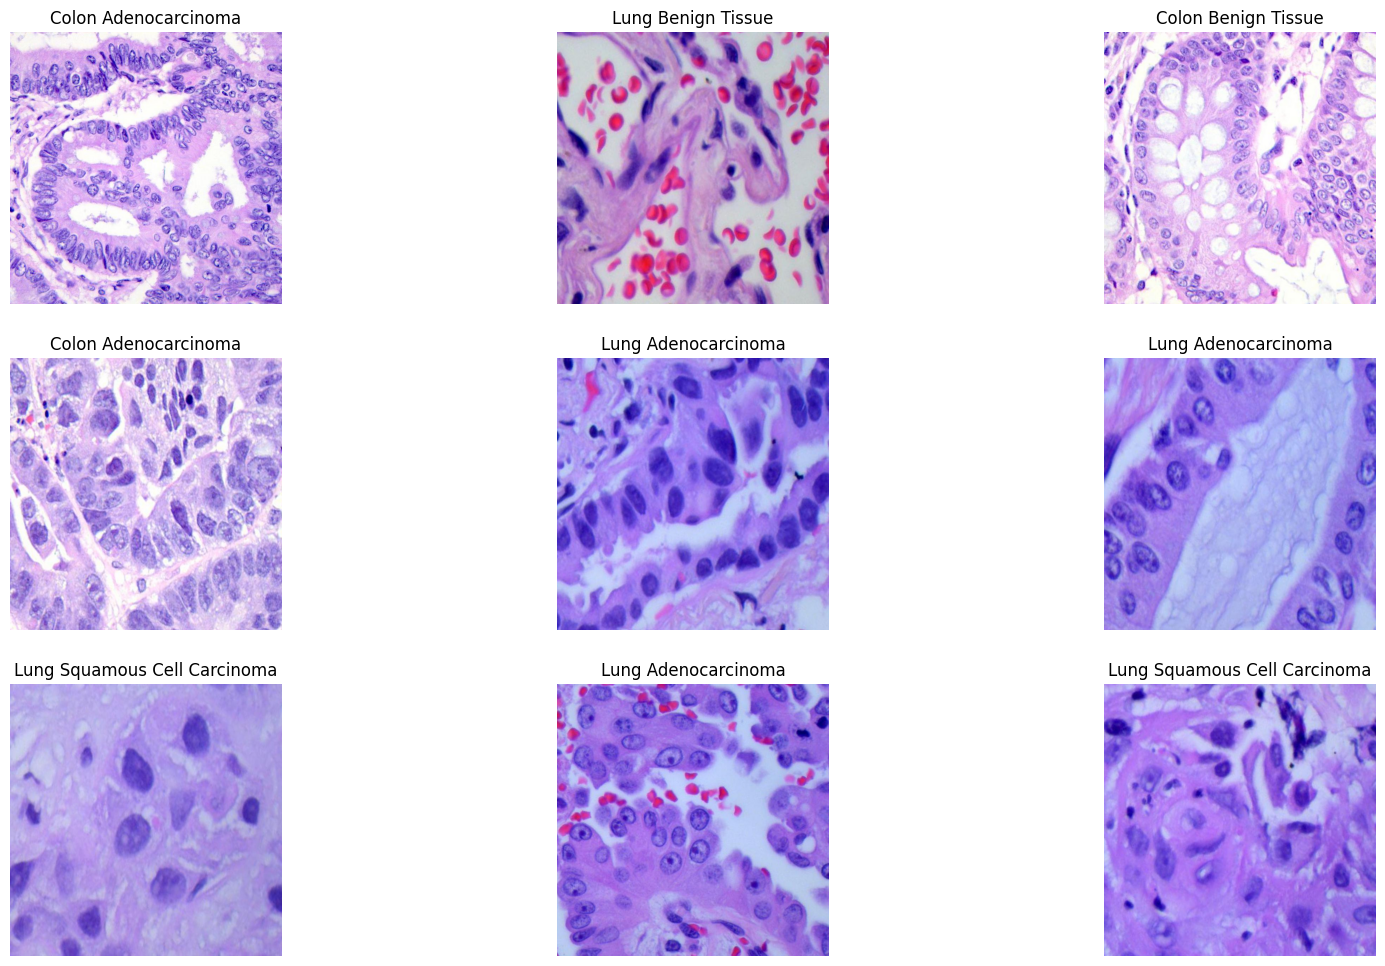
\includegraphics[width=\columnwidth]{ostalo/slike_tkiva.png}
	\caption{Prikaz 9 slučajno odabranih slika tkiva iz skupa podataka}
	\label{fig:tissue_images}
\end{figure}


\section{Opis našeg rješenja}
Skup podataka \textit{LC25000} podijeljen je na 3 disjunktna podskupa: skup za učenje (70\% podataka), skup za validaciju (10\% podataka) i skup za testiranje ((20\% podataka)).. Dodatno, prilikom učenja korištene su minigrupe od po 16 slika. Korištena su 2 modela: \textit{ResNet50} i \textit{MobileNetV2}. 

\subsection{Konvolucijske neuronske mreže}

TODO opisati što to je konvolucijska mreža i konvolucijski sloj



\subsection{ResNet50}
Konvolucijska neuronska mreža s 50 slojeva \textit{ResNet50} korištena je kao temelj prvog modela.



TODO što to je ResNet50, po čemu je poseban
Validacijski skup za odabir najboljeg modela



 Prednaučena je na skupu podataka \textit{ImageNet}. Dodano je još 4 skrivena te 1 jedan izlazni sloj. Skriveni slojevi su redom: \textit{BatchNormalization}, \textit{Flatten}, \textit{Dense} s aktivacijskom funkcijom \textit{ReLu} i \textit{Dropout}. Izlazni sloj je \textit{Dense} s aktivacijskom funkcijom \textit{softmax}.

Dakle model \textit{ResNet50} ima 55 slojeva i 49287557 parametara, od kojih je 25695749 njih učivo. Učenje modela provedeno je kroz 60 epoha.


\subsection{MobileNetV2}
Konvolucijska neuronska mreža s 53 sloja \textit{MobileNetV2} korištena je kao temelj drugog modela.



TODO što to je MobileNetV2, po čemu je poseban
 Napomenuti da se trenirala cijela mreža (za razliku od resnet50a, manje parametara)



 Prednaučena je na skupu podataka \textit{ImageNet}. Dodano je još 2 skrivena te 1 izlazni sloj. Skriveni slojevi su  \textit{BatchNormalization} i \textit{Flatten}. Izlazni sloj je \textit{Dense} s aktivacijskom funkcijom \textit{softmax}.

Dakle model \textit{MobileNetV2} ima 56 slojeva i 2576709 parametara, od kojih je 2540037 njih učivo. Učenje modela provedeno je kroz 60 epoha.



\section{Rezultati}

\subsection{Točnost i gubitak}
Za oba modela prikazani su grafovi točnosti i gubitka na skupu za učenje i skupu za validaciju tijekom procesa učenja (slike \ref{fig:RN50_acc_loss} i \ref{fig:MN_acc_loss}). 
\begin{figure}[ht]
	\centering
	\includegraphics[width=\columnwidth]{ResNet50/accuracy_loss.png}
	\caption{Točnost (lijevo) i gubitak (desno) modela ResNet50 nad podacima za treniranje i validaciju po epohama}
	\label{fig:RN50_acc_loss}
\end{figure}
\begin{figure}[ht]
	\centering
	\includegraphics[width=\columnwidth]{MobileNetV2/accuracy_loss.png}
	\caption{Točnost (lijevo) i gubitak (desno) modela MobileNetV2 nad podacima za treniranje i validaciju po epohama}
	\label{fig:MN_acc_loss}
\end{figure}

Tablicom \ref{table:1} usporedno su prikazane točnosti predviđanja, a tablicom \ref{table:2} gubici oba modela  nakon učenja. Točnosti i gubici odnose se na predviđanja nad skupom za učenje, skupom za validaciju i skupom za testiranje. 

%Primjetno je da model \textit{ResNet50} ima veću točnost (99.32\%) na skupu za testiranje od modela \textit{MobileNetV2} (98.65\%).

\begin{table}[ht]
	\centering
		\caption{Točnosti modela}
	\label{table:1}
\begin{tabular}{ |c|c|c|c| } 
	\hline
	& \multicolumn{3}{c|}{Točnost} \\
	\hline
	Model & Skup za učenje & Skup za validaciju & Skup za testiranje \\
	\hline \hline
	ResNet50 & 99.45\% & 98.96\% & 99.32\%  \\
	\hline
	MobileNetV2 & 99.78\% & 97.49\% & 98.65\%  \\
	\hline
	\end{tabular}
\end{table}
\begin{table}[ht]
	\centering
	\caption{Gubici modela}
	\label{table:2}
	\begin{tabular}{ |c|c|c|c| } 
		\hline
		& \multicolumn{3}{c|}{Gubitak} \\
		\hline
		Model & Skup za učenje & Skup za validaciju & Skup za testiranje \\
		\hline \hline
		ResNet50 & 0.049 & 0.152 & 0.091  \\
		\hline
		MobileNetV2 & 0.011 & 0.100 & 0.047 \\
		\hline
	\end{tabular}
\end{table}



\pagebreak

\subsection{Matrica zabune}
Matrica zabune, računata na skupu za testiranje, prikazana je za oba modela (slike \ref{fig:RN50_conf_mat} i \ref{fig:MN_conf_mat}).

Radi lakšeg snalaženja na matrici zabune, u tablici \ref{table:3} predstavljene su brojčane oznake pojedinih razreda.

\begin{table}[ht]
	\centering
	\caption{Oznake razreda na grafu}
	\label{table:3}
	\begin{tabular}{ |c|c| } 
		\hline
		Oznaka & Razred \\
		\hline \hline
		0 & Adenokarcinom tkiva debelog crijeva \\
		\hline
		1 & Dobroćudno (benigno) tkivo debelog crijeva \\
		\hline
		2 & Adenokarcinom plućnog tkiva \\
		\hline
		3 & Dobroćudno (benigno) plućno tkivo \\
		\hline
		4 & Karcinom pločastih (skvamoznih) stanica plućnog tkiva \\
		\hline
	\end{tabular}
\end{table}


\begin{figure}[ht]
	\centering
	\includegraphics[width=\columnwidth]{ResNet50/confusion_matrix.png}
	\caption{Matrica zabune modela ResNet50}
	\label{fig:RN50_conf_mat}
\end{figure}


\begin{figure}[ht]
	\centering
	\includegraphics[width=\columnwidth]{MobileNetV2/confusion_matrix.png}
	\caption{Matrica zabune modela MobileNetV2}
	\label{fig:MN_conf_mat}
\end{figure}
\pagebreak

%Matrice zabune oba modela su slične, ali \textit{ResNet50} ima točnije predviđanje za razrede 1 i 2 te bitno točnije predviđanje za razred 4 (Karcinom pločastih (skvamoznih) stanica plućnog tkiva).


\section{Mjere dobrote}
 Konačno, za svaki razred u oba modela dan je stupčasti dijagram sljedećih mjera dobrote: točnost (\ref{eq:1}), preciznost (\ref{eq:2}), F1 (\ref{eq:4}), odziv (\ref{eq:3}) i specifičnost (\ref{eq:5}) (slike \ref{fig:RN50_fit_met} i \ref{fig:MN_fit_met}).

\begin{equation}
	Accuracy = \frac{TP + TN}{TP + TN + FP + FN} \label{eq:1}
\end{equation}
\begin{equation}
	Precision = \frac{TP}{TP + FP} \label{eq:2}
\end{equation}
\begin{equation}
	Recall = \frac{TP}{TP + FN} \label{eq:3}
\end{equation}
\begin{equation}
	F1 = \frac{TP}{TP + 0.5(FN + FP)}
\end{equation}
\begin{equation}
	Specificity = \frac{TN}{TN + FP} \label{eq:5}
\end{equation}


\begin{figure}[ht]
	\centering
	\includegraphics[width=\columnwidth]{ResNet50/fitness_metrics.png}
	\caption{Mjere dobrote modela ResNet50}
	\label{fig:RN50_fit_met}
\end{figure}



\begin{figure}[ht]
  \centering
  \includegraphics[width=\columnwidth]{MobileNetV2/fitness_metrics.png}
  \caption{Mjere dobrote modela MobileNetV2}
  \label{fig:MN_fit_met}
\end{figure}
\pagebreak
Isti podaci prikazani su tablično (tablice \ref{table:4} i \ref{table:5}).

\begin{table}[ht]
	\centering
	\caption{Mjere dobrote za model ResNet50}
	\label{table:4}
	\begin{tabular}{ |c|c|c|c|c|c| } 
		\hline
		Oznaka razreda & Točnost & Preciznost & F1 & Odziv & Specifičnost \\
		\hline\hline
		  0 & 99.92\% & 100\% & 99.8\% & 99.6\% & 100\% \\
									\hline
									  1 & 99.92\% & 99.58\% & 99.79\% & 100\% & 99.9\% \\
									 \hline
									  2 & 99.4\% & 98.27\% & 98.47\% & 98.67\% & 99.58\% \\
									 \hline
									  3 & 99.98\% & 100\% & 99.95\% & 99.9\% & 100\% \\
									 \hline
									  4 & 99.98\% & 100\% & 99.95\% & 99.9\% & 100\% \\
									 \hline
	\end{tabular}
\end{table}
\begin{table}[ht]
	\centering
	\caption{Mjere dobrote za model MobileNetV2}
	\label{table:5}
	\begin{tabular}{ |c|c|c|c|c|c| } 
		\hline
		Oznaka razreda & Točnost & Preciznost & F1 & Odziv & Specifičnost \\
		\hline\hline
		0 & 99.62\% & 100\% & 99.05\% & 98.12\% & 100\% \\
		\hline
		1 & 99.82\% & 99.07\% & 99.53\% & 100\% & 99.78\% \\
		\hline
		2 & 98.94\% & 98.57\% & 97.34\% & 96.13\% & 99.65\% \\
		\hline
		3 & 100\% & 100\% & 100\% & 100\% & 100\% \\
		\hline
		4 & 98.94\% & 95.72\% & 97.37\% & 99.09\% & 98.9\% \\
		\hline
	\end{tabular}
\end{table}




\section{Diskusija rezultata i usporedba s prijašnjim radovima}
TODO



\section{Zaključak}
TODO

\bibliography{literatura}
\bibliographystyle{ieeetr}
\end{document}
